\chapter{Sistemas a eventos discretos}
\label{cap:seds}

Segundo \citeonline[p. 142, tradução do autor]{lafortune} \begin{citacao} Sistemas a eventos discretos (\acs{SED}s) são sistemas dinâmicos com duas características definidoras: seus espaços de estados são discretos e potencialmente infinitos, e sua dinâmica é orientada a eventos, em vez de tempo. (...) Eventos que ocorrem de forma assíncrona (em geral) causam um salto no espaço de estados, de um estado para outro. \end{citacao} \citeonline{cassandras} argumentam que os SEDs, diferentemente dos sistemas orientados pelo tempo e governados pelas leis da natureza, não podem ser modelados e estudados usando equações diferenciais. Os SEDs requerem outras técnicas de análise, ferramentas de projeto, métodos de teste, entre outros.

O advento das tecnologias de comunicação, sensoriamento e computação impulsionou a caracterização desta nova classe de sistemas. Os SEDs, por não serem adequadamente modelados pelas equações das leis da física clássica e moderna, demandam novos paradigmas de modelagem. ``Intuitivamente, nós podemos pensar em um modelo como um dispositivo que simplesmente duplica o comportamento do próprio sistema'' \cite[p. 3, tradução do autor]{cassandras}. Um modelo descreve um sistema sob uma ótica quantitativa, que é, muitas vezes, mais adequada que uma simples e subjetiva descrição qualitativa. A construção de um modelo considera um conjunto de variáveis de entrada e saída, relacionadas por intermédio de uma função. Assim sendo, os modelos proporcionam a habilidade predizer os comportamentos de sistemas, o que os confere importância. Formas de modelar sistemas que evoluem com base em eventos assíncronos e discretos são discutidas neste capítulo.

\citeonline{cassandras} citam, como exemplos de SEDs, os sistemas de filas, computacionais, de comunicação, de manufatura e de tráfego. A exemplo disso, protocolos de comunicação em redes de computadores são frequentemente modelados por SEDs, como indica a Figura \ref{fig:protocolo_rede}. O presente trabalho enfoca os sistemas relacionados à automação industrial, para os quais a modelagem de filas é conveniente. A espera de entidades por um recurso em uma fábrica é exemplo que justifica isso, porque a abstração por meio de filas ou \textit{buffers} é muito útil nesse caso. O capítulo \ref{cap:filas} explanará essa e outras situações em que podemos abstrair a noção de filas.

\figura{Protocolo para um canal de redes de computadores com erros de bits: lado remetente e (abaixo) destinatário}{
	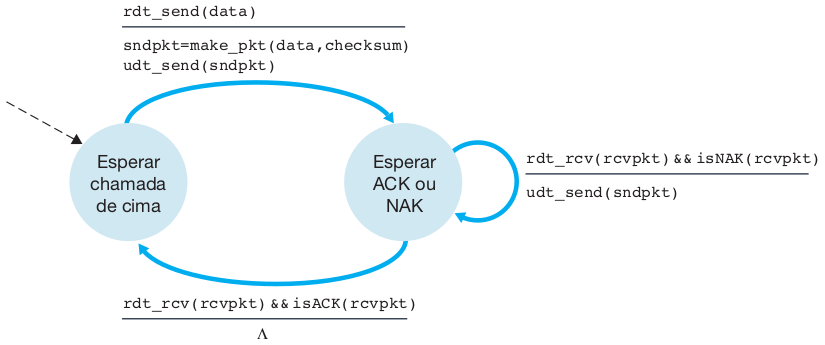
\includegraphics[width=.9 \textwidth]{figuras/rdt2_0-remetente.png}\\
	\vspace{8mm}
	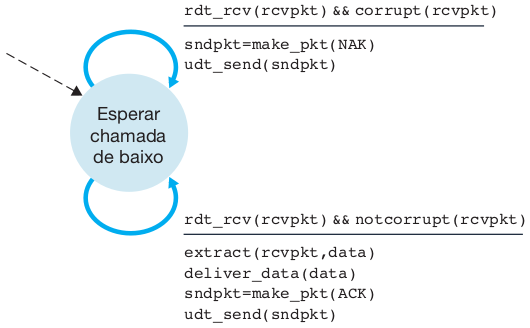
\includegraphics[width=.6 \textwidth]{figuras/rdt2_0-destinatario.png}
}{fig:protocolo_rede}{KUROSE, J.; ROSS K. \textbf{Redes de computadores e a internet}: uma abordagem top-down. 6. ed. São Paulo: Pearson, 2013}

Na figura \ref{fig:protocolo_rede}, tem-se representado um protocolo de redes em que há estados de espera e transições que dependem de eventos discretos -- neste caso, procedimentos computacionais. A representação supracitada é uma evidência do caráter de SED do protocolo, e a figura é um diagrama de estados, que será introduzido mais adiante.

SEDs são comumente modelados por redes de Petri e autômatos determinísticos. Redes de Petri são uma classe de grafos direcionados que têm duas variedades de nós: posições e transições. Nelas, os arcos podem ligar dois nós apenas se forem diferentes -- não pode haver arcos entre duas posições, por exemplo -- e têm pesos que indicam a quantidade de tokens que serão consumidos ou produzidos. Geralmente, os tokens, posições e transições representam recursos, condições e eventos respectivamente e permitem modelar atividades paralelas, protocolos de comunicação, sistemas de produtor-consumidor com prioridade, etc. \cite{petrinets} Este trabalho de conclusão de concurso, todavia, tem enfoque na representação por autômatos finitos determinísticos. A seção \ref{sec:afd}, que segue, introduz os principais conceitos desses modelos.

\section{Autômatos finitos determinísticos}
\label{sec:afd}

Autômato -- palavra derivada do termo em latim \textit{automatu} -- é ``maquinismo que se move por meios mecânicos'' e ``imita os movimentos humanos'' \cite[p. 81]{aurelio}. Esse termo tem sido usado na ciência da computação desde a década de 1930 para descrever importantes modelos da Teoria dos Autômatos, que aborda máquinas de Turing, por exemplo. Nesse contexto, um autômato é uma máquina abstrata descrita matematicamente e idealizada em termos de limitações físicas \cite{hopcroft}.

Um autômato finito determinístico (\acs{AFD}), ou máquina de estados finitos determinística, é uma máquina dotada de fita, unidade de controle e função de transição. A fita de um autômato é um espaço ilimitado utilizado para armazenar uma sequência de símbolos que serão lidos e computados. Já a unidade de controle contém as variáveis do estado atual da máquina, que servem de parâmetro para a computação da função de transição. Para determinar o estado de um autômato, há uma cabeça de leitura sobre a fita e um conjunto de elementos abstratos que norteiam a evolução do funcionamento da máquina: os estados \cite{hopcroft}. A Figura \ref{fig:afd_componentes} esquematiza a transição de estado de um AFD com a cabeça de leitura inicialmente posicionada sobre a segunda célula da fita.

\figuradoautor{Transição de um AFD}{
    \begin{tikzpicture}
        \draw[draw=black] (0,0.8) rectangle ++(0.8,0.8)
        (0.8,0.8) rectangle ++(0.8,0.8)
        (1.6,0.8) rectangle ++(0.8,0.8)
        (2.4,0.8) rectangle ++(0.8,0.8)
        (3.2,0.8) rectangle ++(0.8,0.8)
        (4.8,0.8) rectangle ++(0.8,0.8)
        (5.6,0.8) rectangle ++(0.8,0.8);
        \draw[>=triangle 60,->,line width=0.6mm] (1.2,0.4) -- (1.2,0.7);
        \node at (1.2,0) {estado $q$};
        \node at (0.4,1.2) {$a_1$};
        \node at (1.2,1.2) {$a_2$};
        \node at (2.0,1.2) {$a_3$};
        \node at (2.8,1.2) {$a_4$};
        \node at (3.6,1.2) {$a_5$};
        \node at (4.4,1.2) {$...$};
        \node at (5.2,1.2) {$a_n$};
        
        \draw[>=triangle 60,->,line width=0.4mm, draw=gray] (6.6,1.2) -- (7.8,1.2);
        
        \draw[draw=black] (8,0.8) rectangle ++(0.8,0.8)
        (8.8,0.8) rectangle ++(0.8,0.8)
        (9.6,0.8) rectangle ++(0.8,0.8)
        (10.4,0.8) rectangle ++(0.8,0.8)
        (11.2,0.8) rectangle ++(0.8,0.8)
        (12.8,0.8) rectangle ++(0.8,0.8)
        (13.6,0.8) rectangle ++(0.8,0.8);
        \draw[>=triangle 60,->,line width=0.6mm] (10.0,0.4) -- (10.0,0.7);
        \node at (10.0,0) {estado $q'$};
        \node at (8.4,1.2) {$a_1$};
        \node at (9.2,1.2) {$a_2$};
        \node at (10.0,1.2) {$a_3$};
        \node at (10.8,1.2) {$a_4$};
        \node at (11.6,1.2) {$a_5$};
        \node at (12.4,1.2) {$...$};
        \node at (13.2,1.2) {$a_n$};
    \end{tikzpicture}
}{fig:afd_componentes}

Durante a computação de uma cadeia de entrada, o AFD lê o símbolo da célula atual da fita, apontada pela cabeça de leitura, e avança o cabeçote em uma posição para a direita. Inicialmente, ao receber uma entrada, a cabeça de leitura estará posicionada na extremidade esquerda da fita e, por conseguinte, da cadeia de símbolos. Se a computação de um símbolo lido não acarretar um estado definido ou a cabeça de leitura estiver posicionada sobre uma célula vazia, o funcionamento do autômato será interrompido.

Na Ciência da Computação, os AFDs formam a base de alguns componentes de software e partes de compiladores. Um artifício muito empregado no desenvolvimento de software são as expressões regulares, que podem ser convertidas em AFDs e permitem encontrar padrões em textos \cite{hopcroft}. Já no contexto dos \acs{SED}s, os AFDs são modelos matemáticos que descrevem sistemas com base nos eventos que podem ocorrer. Dessa maneira, as cadeias de símbolos que são enviadas à entrada dos AFDs constituem sequências de eventos cuja computação resulta em uma descrição do sistema baseada nas variáveis de controle da máquina de estados \cite{cassandras}.

\subsection{Definição formal}

A definição de \acs{AFD} que segue foi inspirada e adaptada de \citeonline{hopcroft} e \citeonline{cassandras}.

Um AFD $G$ é uma quíntupla \begin{equation}
\label{eq:afd}
\langle Q, E, \delta, q_0, Q_m \rangle
\end{equation} em que \begin{itemize}[label={}]
  \item $Q$ é o conjunto finito de estados
  \item $E$ é o conjunto finito de símbolos ou eventos
  \item $\delta:Q \times E \nrightarrow Q$ é a função de transição
  \item $q_0 $ é o estado inicial
  \item $Q_m \subseteq Q$ é o conjunto de estados marcados
\end{itemize}

A função de eventos ativos de $G$, que será denotada por $\Gamma_G:Q \to 2^E$, relaciona cada estado com os eventos possíveis a partir dele. Formalmente, para todo estado $q \in Q$ $$\forall e \in E, e \in \Gamma_G(q) \Leftrightarrow \delta(q, e) \in Q$$ isto é, $e \in \Gamma_G(q)$ se e somente se $\delta(q, e)$ é definido.

Ao fecho de Kleene sobre um conjunto de eventos $E$, denotado por $E^\star$, pertencem todas as possíveis cadeias de eventos pertencentes a $E$. Uma cadeia de eventos é uma sequência finita $e_1 e_2 ... e_{|w|}$ em que $e_i \in E$ ($\forall i = 1..|w|$). Quando $|w| = 0$, a cadeia é dita vazia e será simbolizada por $\varepsilon$.

A função de transição estendida $\hat{\delta}:Q \times E^\star \nrightarrow Q$ é definida recursivamente destarte: $$\hat{\delta}(q, w) = \begin{cases}
q & \text{se $w=\varepsilon$} \\
\hat{\delta}(\delta(q, e), w') & \text{se $w=e w'$}
\end{cases}$$ e terá valor indefinido quando $\delta(q, e)$ assim for.

Embora a formulação matemática de um AFD seja muito útil e importante para formalizar SEDs e provar propriedades destes, a visualização do funcionamento destes autômatos é facilitada com a representação por diagramas de estados. Ademais, tendo em vista que o presente trabalho dispõe de diversos destes diagramas, a subseção seguinte, \ref{subsec:diagramas}, introduz essas representações.

\subsection{Diagrama de estados}
\label{subsec:diagramas}

Para auxiliar na visualização das transições entre os estados dos autômatos, os AFDs são comumente representados por diagramas de estados. Nessa representação, os estados são nós de uma estrutura semelhante a de grafos, e as transições, arestas que interligam dois nós, conforme a Figura \ref{fig:afd_diagrama}. Representam-se as transições cuja origem e destino são o mesmo estado por \textit{loops}: arestas que partem de um nó e terminam no mesmo.

\figuradoautor{Representação da transição de estados em um diagrama}{
    \begin{tikzpicture}[shorten >=1pt,node distance=2cm,on grid,auto] 
        \node[state,minimum size=1.7cm] (q0) {$q$}; 
        \node[state,accepting,minimum size=1.7cm] at (4,0) (q1) {$\delta(q, e)$};
        \draw
        (q0) edge node{$e$} (q1);
    \end{tikzpicture}
}{fig:afd_diagrama}

Nesta classe de diagramas, os estados inicial e final podem ser destacados de alguma forma. Para este trabalho, uma seta sem origem aponta sempre para o nó do estado inicial, e uma circunferência dupla enfatiza o de um estado final, como demonstra a Figura \ref{fig:afd_estado_inicial}.

\figuradoautor{Representação de estados inicial (à esquerda) e final (à direita) em um diagrama}{
    \begin{tikzpicture}[shorten >=1pt,node distance=2cm,on grid,auto] 
        \node[align=center,state,initial] (q0) {estado\\inicial};
        \node[align=center,state,accepting] at (4,0) (qf) {estado\\final};
    \end{tikzpicture}
}{fig:afd_estado_inicial}

Pode-se citar outros aspectos desta representação de autômatos: a possibilidade de adicionar rótulos aos nós, a opção de omitir os nomes dos estados nos nós quando não forem necessários e a aglutinação de transições que partem e terminam no mesmo estado em uma mesma aresta, com os símbolos separados por vírgula.

\subsection{Linguagem marcada}

A linguagem marcada por um AFD $G$ é o conjunto $$L_m(G) = \{ w \in E^\star \mid \hat{\delta}(q_0, w) \in Q_m \}$$ Sendo assim, a linguagem marcada pelo autômato são todas as cadeias de eventos que o fazem transicionar do estado inicial a um estado marcado. Isso significa que, quando uma cadeia $w \in L_m(G)$ for posicionada na fita do autômato, a computação de cada evento, da esquerda para a direita da sequência, sempre resultará em um estado definido e terminará em um estado marcado.

Denomina-se linguagem regular a linguagem marcada por qualquer AFD \cite{hopcroft}. Desse modo, este trabalho de conclusão de curso versará sobre linguagens exclusivamente regulares, a exemplo das quais é possível citar o conjunto dos números naturais pares. Sabendo que um número par é aquele cujo último algarismo -- da esquerda para a direita -- pertence a $\{ 0, 2, 4, 6, 8 \}$, pode-se construir o AFD da Figura \ref{fig:afd_pares}, demonstrando a validade da afirmação.

\figuradoautor{Diagrama de estados para um AFD que reconhece os números naturais pares}{
    \begin{tikzpicture}[shorten >=1pt,node distance=2cm,on grid,auto] 
        \node[state,initial] (q0) {}; 
        \node[state,accepting] at (5,0) (q1) {};
        \draw
            (q0) edge[loop above] node{$1$, $3$, $5$, $7$, $9$} (q0)
            (q0) edge[bend left, above] node{$0$, $2$, $4$, $6$, $8$} (q1)
            (q1) edge[loop above] node{$0$, $2$, $4$, $6$, $8$} (q1)
            (q1) edge[bend left, below] node{$1$, $3$, $5$, $7$, $9$} (q0);
    \end{tikzpicture}
}{fig:afd_pares}

Quando um autômato se destina a verificar padrões em cadeias de eventos, ou palavras, diz-se que ele é um formalismo reconhecedor \cite{menezes} e, portanto, o autômato da Figura \ref{fig:afd_pares} reconhece todos os números naturais pares. No que tange aos \acs{SED}s, alcançar um estado marcado implica a conclusão de alguma tarefa \cite{cassandras}. A impossibilidade de concluir tarefas, os bloqueios ocorrem quando não é possível sair de um estado não marcado e chegar a um marcado, tema da subseção seguinte, \ref{subsec:ling_ger}.

\subsection{Linguagem gerada e bloqueios}
\label{subsec:ling_ger}

A linguagem gerada por um AFD $G$ é o conjunto $$L(G) = \{ w \in E^\star \mid \hat{\delta}(q_0, w) \in Q \}$$ Neste caso, a linguagem são todas as cadeias de eventos que fazem o autômato transicionar do estado inicial a um estado definido.

Caso o autômato $G$ chegue a um estado $q \not\in Q_m$ tal que $\Gamma_G(q) = \varnothing$, diz-se que há um \textit{deadlock}, já que não existe evento que pode ser executado a partir de $q$. Um \textit{livelock} se configura quando, mesmo não havendo \textit{deadlock}, não é possível alcançar um estado marcado. Se qualquer bloqueio acontece $$\overline{L_m(G)} \subset L(G)$$ em que $\overline{L_m(G)}$ é o conjunto de todos os prefixos de todas as cadeias pertencentes a $L_m(G)$, ou $$\overline{L_m(G)} = \{ w \in E^\star \mid \exists w' \in E^\star, w w' \in L_m(G) \}$$ Isso é devido à constatação de que, tendo sido executada uma cadeia de eventos $w \in E^\star$ e estando em um bloqueio, $w$ pertencerá a $L(G)$, mas não será prefixo de alguma cadeia da linguagem marcada: não haverá $w' \in E^\star$ tal que $ww' \in L_m(G)$, por definição \cite{cassandras}.

\subsection{Função de transição total}

Haja vista que não é possível formular funções parciais no assistente de provas Coq, algumas mudanças na definição de AFD supracitada são necessárias a fim de representar AFDs nessa ferramenta. A começar, é impreterível alterar a função de transição de um AFD $G$ para torná-la total. Seja $\delta' : Q \cup \{ \otimes \} \times E \to Q \cup \{ \otimes \}$ a seguinte função total: $$\delta'(q, e) = \begin{cases}
\delta(q, e) & \text{se $\delta(q, e) \in Q$} \\
\otimes & \text{senão}
\end{cases}$$ em que $\otimes$ é um estado novo, não pertencente a $Q$: o estado de ralo.

O autômato $G$ é muito semelhante ao $$G' = \langle Q \cup \{ \otimes \}, E, \delta', q_0, Q_m \rangle$$ uma vez que a única diferença entre eles é que, em $G'$, ao realizar-se uma transição que seria indefinida em $G$, alcança-se um estado do qual não se pode sair.

Como a função $\delta'$ é total, tem-se que $$L(G') = E^\star$$ em termos do que se estabeleceu como linguagem gerada anteriormente. Pode-se, não obstante, modificar a definição dela de forma que $G$ e $G'$ sejam equivalentes em se tratando de linguagens: \begin{equation}
\label{eq:ling_ralo}
L'(G') = \{ w \in E^\star \mid \hat{\delta}(q_0, w) \in Q \wedge \hat{\delta}(q_0, w) \neq \otimes \}
\end{equation} é a linguagem gerada pelo autômato $G'$. Então $$L'(G') = L'(G) = L(G)$$

É possível visualizar as formulações de um AFD usando função de transição parcial e total na Figura \ref{fig:afd_funcao_total}, que a exemplifica para um AFD de alfabeto $\{ a, b \}$.

\figuradoautor{Um AFD simples (à esquerda) e seu correspondente com função de transição total (à direita)}{
	\raisebox{-0.5\height}{\begin{tikzpicture}[shorten >=1pt,node distance=2cm,on grid,auto] 
	\node[state,initial,accepting] (q0) {$q_0$}; 
	\node[state] at (3,0) (q1) {$q_1$};
	\draw
	(q0) edge[bend left, above] node{$a$} (q1)
	(q1) edge[bend left, below] node{$b$} (q0);
	\end{tikzpicture}}
	\raisebox{-0.5\height}{\begin{tikzpicture}[shorten >=1pt,node distance=2cm,on grid,auto] 
	\node[state,initial,accepting] at (0, 2) (q0) {$q_0$}; 
	\node[state] at (3,2) (q1) {$q_1$};
	\node[state] at (1.5,0) (q2) {$\otimes$};
	\draw
	(q0) edge[bend left, above] node{$a$} (q1)
	(q0) edge[bend right, below] node{$b$} (q2)
	(q1) edge[bend left, below] node{$a$} (q2)
	(q1) edge[bend left, below] node{$b$} (q0)
	(q2) edge[loop below] node{$a$, $b$} (q2);
	\end{tikzpicture}}
}{fig:afd_funcao_total}

Isso posto, é evidente que um AFD cuja função de transição não é total pode ser modelado matematicamente utilizando funções totais. Esse fato é importante para que se possa representá-lo na linguagem do Coq.

\subsection{Formulação em Coq}
\label{subsec:afd_coq}

Todas as definições acerca de AFDs supracitadas utilizam conjuntos, mas, para representar os autômatos no assistente de provas Coq, é necessário que sejam usados tipos. Assim, estados e eventos terão tipos específicos.

Conforme a subseção 3.1.5, a formulação de AFDs em Coq precisa considerar o estado de ralo para que a função de transição seja sempre total. Nesse sentido, pode-se definir os estados como do seguinte tipo paramétrico: $$\text{\texttt{Inductive state \{Q : Type\} := sink\_state | proper\_state (q : Q).}}$$ sendo \textit{proper state} -- estado próprio -- qualquer estado do autômato exceto o de ralo. Ao invés de usar apenas o tipo \texttt{Q}, essa definição é importante para facilitar a caracterização das linguagens geradas, já que o estado de ralo tem de estar bem delimitado para defini-las, como demonstra a equação \ref{eq:ling_ralo}.

A função de transição será do tipo \texttt{Q$\to$E$\to$state}, e não \texttt{state$\to$E$\to$state}, o que permitiria quaisquer transições partindo do estado de ralo. Ademais, é importante especificar quais estados são marcados com uma função do tipo \texttt{Q$\to$bool} que retorna \texttt{true} se e somente se o estado for marcado.

Com isso, um autômato determinístico \texttt{g : dfa} terá estes campos: \begin{itemize}
	\item \texttt{Q}: o tipo dos estados próprios
	\item \texttt{E}: o tipo dos símbolos ou eventos
	\item  \texttt{transition : Q$\to$E$\to$@state Q}: a função de transição
	\item \texttt{initial\_state : Q}: o estado inicial
	\item \texttt{is\_marked : Q$\to$bool}: a função de demarcação dos estados
\end{itemize}

Esta definição permite que termos do tipo \texttt{dfa} sejam, com efeito, autômatos infinitos determinísticos. O presente trabalho, porém, assume que os tipos dos estados e eventos são sempre finitos. A implementação do tipo \texttt{dfa} proposta é apresentada pela Figura \ref{fig:dfa_record}.

\figuradoautor{Implementação do tipo dos AFDs em Coq}{
	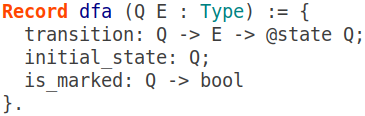
\includegraphics[width=8cm]{figuras/dfa_record.png}
}{fig:dfa_record}

A definição de AFD anterior é equivalente a esta. Sejam $q_1$, $q_2$, $...$ e $q_n$, $q^*$ e $e_1$, $e_2$, $...$ e $e_m$, respectivamente, todos os estados, o estado inicial e todos os possíveis símbolos de um AFD, podemos construir os tipos que seguem: \begin{gather*}\texttt{Inductive Q := $q_1$ | $q_2$ | $...$ | $q_n$.}\\ \texttt{Inductive E := $e_1$ | $e_2$ | $...$ | $e_m$.}\end{gather*} que são os respectivos tipos dos estados e eventos do autômato na definição para o Coq. Seja $\delta : \{ q_1, q_2, ..., q_n \} \times \{ e_1, e_2, ..., e_m \} \nrightarrow \{ q_1, q_2, ..., q_n \}$ a função de transição de estados tal que $$\delta(q, e) = \begin{cases}
q' & \text{se \texttt{transition $q$ $e$ $=$ proper\_state $q'$}}
\end{cases}$$ ou, por outro lado, seja \texttt{transition : Q$\to$E$\to$@state Q} assim definida na linguagem do Coq: 	\begin{align*}
&\texttt{Fixpoint transition (q : Q) (e : E) : state :=}\\
&\texttt{match q, e with}\\
&\texttt{$q'$, $e'$ => proper\_state $\delta(q', e')$ |}\\
&\texttt{\_, \_ => sink\_state}\\
&\texttt{end.}
\end{align*} sendo $x = (q',e')$ todo par tal que $\delta(x)$ é definido. Além disso, determinemos o conjunto de estados marcados: $$Q_m = \{ q_i \mid i \in \{ 1, 2, ..., n \} \wedge \texttt{is\_marked $q_i$ $=$ true} \}$$ ou, de outra parte, construamos a função \texttt{is\_marked}: \begin{align*}
&\texttt{Fixpoint is\_marked (q : Q) : bool :=}\\
&\texttt{match q with}\\
&\texttt{$q_m$ => true |}\\
&\texttt{\_ => false}\\
&\texttt{end.}
\end{align*} em que $q_m$ é todo estado pertencente a $Q_m$. Portanto, o autômato $\langle \{ q_1, q_2, ..., q_n \}, \{ e_1, e_2, ..., e_m \}, \delta, q^*, Q_m \rangle$ pode ser formulado em termos dos elementos \texttt{Q}, \texttt{E}, \texttt{transition} e \texttt{is\_marked} e vice-versa.

Toda sequência de eventos será representada por uma lista, e a função de transição estendida \texttt{extended\_transition} será do tipo \texttt{dfa$\to$@state Q$\to$list E$\to$@state Q} e definida recursivamente. Se o estado de origem for o de ralo, ele será o próprio retorno da função; senão, \texttt{extended\_transition} computará a função de transição para a cabeça da lista de eventos e fará recursão destarte: \begin{gather*}
\texttt{extended\_transition g (proper\_state q) [] = proper\_state q;}\\\texttt{extended\_transition g (proper\_state q) e::w =}\\\texttt{extended\_transition g (transition q e) w}\end{gather*}

Por definição, uma lista de eventos \texttt{w} será gerada por \texttt{g}, ou \texttt{g ==> w}, se $$\texttt{extended\_transition g (proper\_state initial\_state) w $\neq$ sink\_state}$$ ou seja, se a computação da função de transição estendida da lista partindo do estado inicial não resultar no estado de ralo, em conformidade com a equação \ref{eq:ling_ralo}. Sendo $G$ o AFD definido conforme a equação \ref{eq:afd} e equivalente ao \texttt{g}, podemos notar $$L(G) = \{ a_1a_2...a_n \in E^\star \mid \texttt{g ==> [$a_1$;$a_2$;$...$;$a_n$]} \}$$ evidenciando também a correlação entre as diferentes definições supracitadas para a mesma classe de máquinas abstratas.